\section{Zielsetzung}

Ziel dieses Versuches ist es, mithilfe eines Michelson-Interferometer die Wellenlänge
eines Lasers zu bestimmen sowie über Druckvariation den Brechungsindex von Luft zu bestimmen.

\section{Theorie}
\label{sec:Theorie}

\subsection{Interferenz und Kohärenz}

Licht ist eine elektromagnetische Welle und wird mathematisch somit durch die Lösung einer Wellengleichung beschrieben:
\begin{equation*}
    \vec{E}(x,t) = \vec{E_0} \cos(kx-wt-\delta),
\end{equation*}

Wie allgemein von allen Wellenphänomenen bekannt, können aufeinandertreffende Wellen superponiert werden,
dabei entsteht sogenannte Inteferenz.
Bei identischer Phase addieren sich die Amplituden und es liegt konstruktive Inteferenz vor, während ein
Phasenversatz von $\frac{\lambda}{2}$ zu einer Auslöschung, auch destruktive Inteferenz genannt, führt.
Aufgrund der sehr großen Frequenz von Licht ist eine Messung der Feldstärke $\vec{E}$ ausgeschlossen, stattdessen
wird die Intensität betrachtet, für die gilt:
\begin{equation*}
    I = \text{const}\lvert \vec{E} \rvert^2
\end{equation*}

Die Intensität von zwei überlagerten Lichtwellen mit Phasen $\delta_1$ und $\delta_2$ ergibt sich dann zu
\begin{equation*}
    I_\text{Ges} = 2 \text{const}\vec{E}_0^2(1 + \cos(\delta_2 - \delta_1))
\end{equation*}

Wichtig ist hierbei, dass die Phasenversätze $\delta_i$ konstant bleiben, also zeitunabhängig sind.
Nur dann kann über messbare Zeiträume eine Intensität bestimmt werden, die auf konstruktive oder destruktive
Inteferenz schließen lässt.
Solches Licht nennt man kohärent, und diese Eigenschaft ist zwingend nötig um Untersuchungen
mit optischen Aufbauten durchzuführen.
Am einfachsten lässt sich kohärentes Licht mithilfe von Lasern erzeugen, da diese monochromatische Lichtbündel
mit konstanter Phase emmitieren.
In sogenannten Interferometern werden Lichtbündel dann gespalten und auf unterschiedliche Wege wieder zusammengeführt,
um Inteferenzphänomene beobachten zu können.


\subsection{Michelson Interferometer}
\label{sec:Michelson Interferometer}

Der schematische Aufbau des 1882 von A. Michelson erfundenen Michelson-Inteferometer ist in
\autoref{fig:Michelson} dargestellt.

\begin{figure}[H]
    \centering
    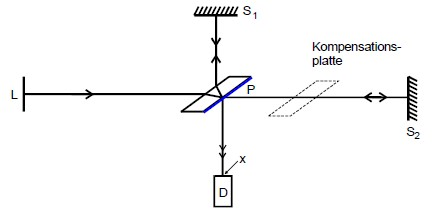
\includegraphics[height=6cm]{content/pics/Michelson.jpg}
    \caption{Schematischer Aufbau eines Michelson Interferometers \cite{v401}.}
    \label{fig:Michelson}
\end{figure}

Der Lichtstrahl aus einer Quelle L wird zuerst durch eine semipermeable Platte P geteilt und somit in zwei Bündel gespalten,
welche sich senkrecht zueinander weiterbewegen.
Die beiden Teilbündel fallen auf zwei Spiegel $\text{S}_1$ und $\text{S}_2$ und werden zurückgeworfen.
Somit treffen die Strahlen wieder in P aufeinander.
Von jedem Strahl wird jeweils ein Teil transmittiert, diese Teilbündel laufen abschließend parallel zueinander zum
Detektor D.
Damit die erwähnten Teilbündel kohärent sind, werden die Längen der beiden Arme möglichst gleich gewählt.
Im Strahlenweg zum Spiegel $\text{S}_2$ muss eine Kompensationsplatte platziert werden, da der Strahl durch
$\text{S}_1$ zwei mal mehr durch die semipermeable Platte P hindurch läuft. Dementsprechend hat die Kompensationsplatte
die selbe Dicke und den selben Brechungsindex wie wie P.

Wählt man identische Armlängen, so löschen sich die Lichtstrahlen am Detektor aus, da bei der Reflexion des von
$\text{S}_2$ kommenden Lichtstrahls an P ein Phasensprung von $\frac{\lambda}{2}$ auftritt.
Durch kontinuierliches Verschieben von einem der Spiegel um ein Stück $d$ kann ein Wegunterschied $w=2d$ erzeugt werden,
die Intensität am Detektor wechselt dann fortlaufend aufgrund von konstruktiver und destruktiver Interferenz
zwischen Null und einem Maximum. Deren räumlicher Abstand beträgt $\frac{\lambda}{2}$, bei $z$ auftretenden
Maxima während einer Verschiebung um $\symup{\Delta}d$ gilt somit der Zusammenhang
\begin{equation}
    \label{eq:Lambda}
    \symup{\Delta}d=z \cdot \frac{\lambda}{2}.
\end{equation}

Ausgenommen der Variation einer der Armlänge besteht eine andere Möglichkeit einen optischen Wegunterschied zu erreichen darin,
den Brechungsindex $n$ in einem der Arme zu variieren.
Es wird also in einem Arm ein Medium der Länge $b$ mit Brechungsindex $n+\symup{\Delta}n$ hinzugefügt, die
neue Anordnung ist in \autoref{fig:Brechung} dargestellt.
\begin{figure}[H]
    \centering
    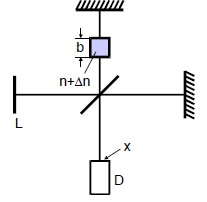
\includegraphics[height=6cm]{content/pics/Brechung.jpg}
    \caption{Inteferenz am Michelson-Interferometer über Brechungsindexunterschiede \cite{v401}.}
    \label{fig:Brechung}
\end{figure}
Für den optischen Wegunterschied gilt nun der Zusammenhang
\begin{equation}
    \label{eq:Delta N}
    b \cdot \symup{\Delta}n=z \cdot \frac{\lambda}{2}.
\end{equation}

\subsection{Druckabhängigkeit des Brechungsindex}

Die Lichtwellen im Inteferometer werden auch durch die Luft, die sich überall im Interferometer befindet,
gebrochen. Bei den vorherigen Betrachtungen ist der Luftdruck konstant, daher hat diese Tatsache
keinen Einfluss auf die Inteferenz im Inteferometer.
Wird jedoch der Druck variert, so ändert sich der Brechungsindex $n$ in Luft und damit auch die Interferenz.
Der neue Brechungsindex lässt sich unter Normalbedingungen ($p_0=\qty{1013.2}{\milli\bar}$ und $T_0=\qty{273.15}{\kelvin}$)
über die folgende Beziehung berechnen
\begin{equation}
    \label{eq:Brechung}
    n(p_0, T_0) = 1 + \symup{\Delta} n(p,p')\frac{T}{T_0}\frac{p_0}{p - p'}.
\end{equation}

Dabei ist die Änderung des Brechungsindex $\symup{\Delta} n(p,p')$ bereits in \autoref{sec:Michelson Interferometer} mit
\eqref{eq:Delta N} beschrieben, sie hängt von der Länge $b$ der Region mit verändertem Druck und der
Wellenlänge $\lambda$ ab.